%% Topology of ternary complex dimer identical
%% FigS3TCDimerTreeTopologyAlternative.tex
%% Unused packages and definitions removed; TikZ/PGFPlots source formatted.

\documentclass{standalone}

\usepackage{amsmath}
\usepackage{tikz}
\usetikzlibrary{arrows}

\def \half {\frac{1}{2}}

\def\b{\mathsf{b}}
\def\c{\mathsf{c}}
\def\d{\mathsf{d}}
\def\x{\mathsf{x}}

\def\kappab{\kappa_{\b}}
\def\kappac{\kappa_{\c}}
\def\kappad{\kappa_{\d}}
\def\kappax{\kappa_{\x}}

\def\etabb{\eta_{\b\b}^{}}
\def\etabc{\eta_{\b\c}^{}}
\def\etacc{\eta_{\c\c}^{}}
\def\etabx{\eta_{\b\x}^{}}
\def\etacx{\eta_{\c\x}^{}}
\def\etaxx{\eta_{\x\x}^{}}

\begin{document}

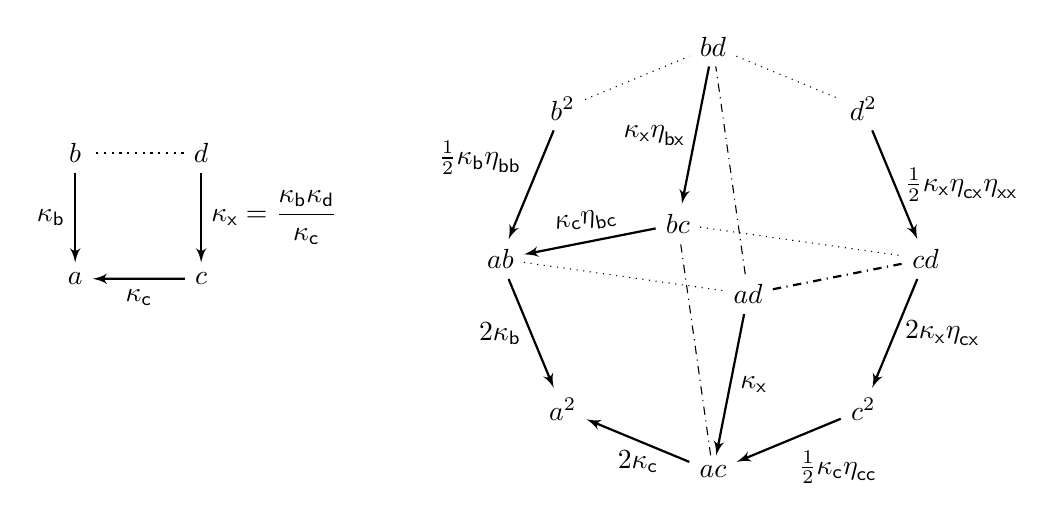
\begin{tikzpicture}[scale=0.9,style=thick,shorten >=0pt,shorten <=0pt,>=latex']
    \begin{scope}[node distance=1.6cm,xshift=-9cm,yshift=1.5cm]
        \node (B) {$b$};
        \node[below of=B] (A) {$a$};
        \draw[->,thick] (B) to node[left,align=center] {$\kappab$} (A);
        \node[right of=A] (C) {$c$};
        \draw[<-,thick] (A) to node[below] (KC) {$\kappac$} (C);
        \node[right of=B] (D) {$d$};
        \draw[dotted] (D) to node[above] {} (B);
        %\path (B) to node[above,yshift=0.8cm] {$T \subset H $} (D);
        \draw[<-,thick] (C) to node[right] {$\kappax = \dfrac{\kappab\kappad}{\kappac}$} (D);
        %\node[below of=KC]{$\kappa_x=\kappa_b\kappa_d/\kappa_c$};
    \end{scope}

    \begin{scope}[xshift=0cm,yshift=0cm,scale=1,shorten >=0pt,shorten <=0pt]
        %\coordinate (title) at (90:3.75);
        %\draw (title) node {$T^{(2)} \subset H^{(2)}$};
        \draw (0:3) node[] (cd) {$cd$};
        \draw (45:3) node[] (d2) {$d^2$};
        \draw (90:3) node[] (bd) {$bd$};
        \draw (135:3) node[] (b2) {$b^2$};
        \draw (180:3) node[] (ab) {$ab$};
        \draw (225:3) node[] (a2) {$a^2$};
        \draw (270:3) node[] (ac) {$ac$};
        \draw (315:3) node[] (c2) {$c^2$};
        \draw (315:0.7) node[] (ad) {$ad$};
        \draw (135:0.7) node[] (bc) {$bc$};
        \draw[<-,thick] (a2) -- node[left] {$2\kappab$} (ab);
        \draw[<-,thick] (ab) -- node[above left] {$\half\kappab\etabb$} (b2);
        \draw[thin,dotted] (b2) -- (bd);
        \draw[thin,dotted] (bd) -- (d2);
        \draw[->,thick] (d2) -- node[right] {$\half \kappax \etacx \etaxx$} (cd);
        \draw[->,thick] (cd) -- node[right] {$2\kappax \etacx$} (c2);
        \draw[<-,thick] (ac) -- node[below right] {$\half\kappac \etacc$} (c2);
        \draw[->,thick] (ac) -- node[below] {$2\kappac$} (a2);
        \draw[<-,thick] (bc) -- node[left] {$\kappax\etabx$} (bd);
        \draw[thin,dashdotted] (ad) -- node[pos=0.75] (adbd) {} (bd);
        \draw[->,thick] (ad) -- node[right] {$\kappax$} (ac);
        \draw[thin,dashdotted] (ac) -- node[pos=0.75] (bcac) {} (bc);
        \draw[<-,thick] (ab) --  node[above,sloped] {$\kappac \etabc$} (bc);
        \draw[thin,dotted] (bc) -- (cd);
        \draw[thin,dashdotted,thick] (ad) -- (cd);
        \draw[thin,dotted] (ab) -- (ad);

    \end{scope}

\end{tikzpicture}

\end{document}

